% Template for PLoS
% Version 3.1 February 2015
%
% To compile to pdf, run:
% latex plos.template
% bibtex plos.template
% latex plos.template
% latex plos.template
% dvipdf plos.template
%
% % % % % % % % % % % % % % % % % % % % % %
%
% -- IMPORTANT NOTE
%
% This template contains comments intended 
% to minimize problems and delays during our production 
% process. Please follow the template instructions
% whenever possible.
%
% % % % % % % % % % % % % % % % % % % % % % % 
%
% Once your paper is accepted for publication, 
% PLEASE REMOVE ALL TRACKED CHANGES in this file and leave only
% the final text of your manuscript.
%
% There are no restrictions on package use within the LaTeX files except that 
% no packages listed in the template may be deleted.
%
% Please do not include colors or graphics in the text.
%
% Please do not create a heading level below \subsection. For 3rd level headings, use \paragraph{}.
%
% % % % % % % % % % % % % % % % % % % % % % %
%
% -- FIGURES AND TABLES
%
% Please include tables/figure captions directly after the paragraph where they are first cited in the text.
%
% DO NOT INCLUDE GRAPHICS IN YOUR MANUSCRIPT
% - Figures should be uploaded separately from your manuscript file. 
% - Figures generated using LaTeX should be extracted and removed from the PDF before submission. 
% - Figures containing multiple panels/subfigures must be combined into one image file before submission.
% For figure citations, please use "Fig." instead of "Figure".
% See http://www.plosone.org/static/figureGuidelines for PLOS figure guidelines.
%
% Tables should be cell-based and may not contain:
% - tabs/spacing/line breaks within cells to alter layout or alignment
% - vertically-merged cells (no tabular environments within tabular environments, do not use \multirow)
% - colors, shading, or graphic objects
% See http://www.plosone.org/static/figureGuidelines#tables for table guidelines.
%
% For tables that exceed the width of the text column, use the adjustwidth environment as illustrated in the example table in text below.
%
% % % % % % % % % % % % % % % % % % % % % % % %
%
% -- EQUATIONS, MATH SYMBOLS, SUBSCRIPTS, AND SUPERSCRIPTS
%
% IMPORTANT
% Below are a few tips to help format your equations and other special characters according to our specifications. For more tips to help reduce the possibility of formatting errors during conversion, please see our LaTeX guidelines at http://www.plosone.org/static/latexGuidelines
%
% Please be sure to include all portions of an equation in the math environment.
%
% Do not include text that is not math in the math environment. For example, CO2 will be CO\textsubscript{2}.
%
% Please add line breaks to long display equations when possible in order to fit size of the column. 
%
% For inline equations, please do not include punctuation (commas, etc) within the math environment unless this is part of the equation.
%
% % % % % % % % % % % % % % % % % % % % % % % % 
%
% Please contact latex@plos.org with any questions.
%
% % % % % % % % % % % % % % % % % % % % % % % %

\documentclass[10pt,letterpaper]{article}
\usepackage[top=0.85in,left=2.75in,footskip=0.75in]{geometry}

% Use adjustwidth environment to exceed column width (see example table in text)
\usepackage{changepage}

% Use Unicode characters when possible
\usepackage[utf8]{inputenc}

% textcomp package and marvosym package for additional characters
\usepackage{textcomp,marvosym}

% fixltx2e package for \textsubscript
\usepackage{fixltx2e}

% amsmath and amssymb packages, useful for mathematical formulas and symbols
\usepackage{amsmath,amssymb}

% cite package, to clean up citations in the main text. Do not remove.
\usepackage{cite}

% Use nameref to cite supporting information files (see Supporting Information section for more info)
\usepackage{nameref,hyperref}

% line numbers
\usepackage[right]{lineno}

% ligatures disabled
\usepackage{microtype}
\DisableLigatures[f]{encoding = *, family = * }

% rotating package for sideways tables
\usepackage{rotating}

% Remove comment for double spacing
\usepackage{setspace} 
\doublespacing

% Text layout
\raggedright
\setlength{\parindent}{0.5cm}
\textwidth 5.25in 
\textheight 8.75in

% Bold the 'Figure #' in the caption and separate it from the title/caption with a period
% Captions will be left justified
\usepackage[aboveskip=1pt,labelfont=bf,labelsep=period,justification=raggedright,singlelinecheck=off]{caption}

% Use the PLoS provided BiBTeX style
\bibliographystyle{plos-latex-template/plos2015}


% Remove brackets from numbering in List of References
\makeatletter
\renewcommand{\@biblabel}[1]{\quad#1.}
\makeatother

% Leave date blank
\date{}

% Header and Footer with logo
\usepackage{lastpage,fancyhdr,graphicx}
\usepackage{epstopdf}
\pagestyle{myheadings}
\pagestyle{fancy}
\fancyhf{}
\lhead{
\includegraphics[width=2.0in]{plos-latex-template/PLOS-submission.eps}}
\rfoot{\thepage/\pageref{LastPage}}
\renewcommand{\footrule}{\hrule height 2pt \vspace{2mm}}
\fancyheadoffset[L]{2.25in}
\fancyfootoffset[L]{2.25in}
\lfoot{\sf PLOS}

%% Include all macros below

\newcommand{\lorem}{{\bf LOREM}}
\newcommand{\ipsum}{{\bf IPSUM}}


%% END MACROS SECTION

%added packages
\usepackage{soul}
\usepackage{color}
%% END ADDED PACKAGES

\begin{document}
\vspace*{0.35in}

% Title must be 250 characters or less.
% Please capitalize all terms in the title except conjunctions, prepositions, and articles.
\begin{flushleft}
{\Large
\textbf\newline{Survey of the Heritability and Sparsity of Gene Expression Traits Across Human Tissues}
}
\newline
% Insert author names, affiliations and corresponding author email (do not include titles, positions, or degrees).
\\
Heather E. Wheeler\textsuperscript{1,2,*},
GTEx Consortium,
Kaanan P. Shah\textsuperscript{3},
. . ., Nancy J. Cox\textsuperscript{4}, Dan L.
Nicolae\textsuperscript{3}, Hae Kyung Im\textsuperscript{3,*}
\\
\bigskip
\bf{1} Department of Biology, Loyola University Chicago, Chicago, IL, USA
\\
\bf{2} Department of Computer Science, Loyola University Chicago, Chicago, IL, USA
\\
\bf{3} Section of Genetic Medicine, Department of Medicine, University of Chicago, Chicago, IL, USA
\\
\bf{4} Division of Genetic Medicine, Vanderbilt University, Nashville, TN, USA
\bigskip

% Insert additional author notes using the symbols described below. Insert symbol callouts after author names as necessary.
% 
% Remove or comment out the author notes below if they aren't used.
%
% Primary Equal Contribution Note
%\Yinyang These authors contributed equally to this work.

% Additional Equal Contribution Note
% Also use this double-dagger symbol for special authorship notes, such as senior authorship.
%\ddag These authors also contributed equally to this work.

% Current address notes
%\textcurrency a Insert current address of first author with an address update
% \textcurrency b Insert current address of second author with an address update
% \textcurrency c Insert current address of third author with an address update

% Deceased author note
%\dag Deceased

% Group/Consortium Author Note
%\textpilcrow Membership list can be found in the Acknowledgments section.

% Use the asterisk to denote corresponding authorship and provide email address in note below.
* hwheeler1@luc.edu, haky@uchicago.edu

\end{flushleft}
% Please keep the abstract below 300 words
\section*{Abstract}
For most complex traits, gene regulation is known to play a crucial mechanistic role as demonstrated by the consistent enrichment of expression quantitative trait loci (eQTLs) among trait-associated variants. Thus, understanding the genetic architecture of gene expression traits is key to elucidating the underlying mechanisms of complex traits. However, a systematic survey of the heritability and the distribution of effect sizes across all representative tissues in the human body has not been reported.

Here we fill this gap through analyses of the RNA-seq data from a comprehensive set of tissue samples generated by the GTEx Project Consortium. We find that local h$^2$ can be relatively well characterized with 2-10\% of expressed genes showing significant h$^2$. However, the current sample sizes ($n<362$) only allow us to compute distal h$^2$ for a handful of genes ($<$0.8\%). In the larger DGN whole blood cohort ($n=922$), 49\% of local h$^2$ estimates are significant, while 3\% of distal h$^2$ estimates are significant. Thus, we focus on local regulation. Bayesian Sparse Linear Mixed Model (BSLMM) analysis and the sparsity of optimal performing predictors provide compelling evidence that local architecture of gene expression traits is sparse rather than polygenic across DGN and all 40 GTEx tissues examined.

To further delve into the tissue context specificity, we decompose the expression traits into cross-tissue and tissue-specific components. Heritability and sparsity estimates of these derived expression phenotypes show similar characteristics to the original traits. Consistent properties relative to prior GTEx multi-tissue analysis results suggest that these traits reflect the expected biology.

Finally, we apply this knowledge to develop prediction models of gene expression traits for all tissues. The prediction models, heritability, and prediction performance R\textsuperscript{2} for original and decomposed expression phenotypes are made publicly available (\url{https://github.com/hakyimlab/PrediXcan}).


% Please keep the Author Summary between 150 and 200 words
% Use first person. PLOS ONE authors please skip this step. 
% Author Summary not valid for PLOS ONE submissions.   
\section*{Author Summary}
Gene regulation is known to contribute to the underlying mechanisms of complex traits. The GTEx project has generated RNA-Seq data on hundreds of individuals across more than 40 tissues providing a comprehensive atlas of gene expression traits. Here, we systematically examined the local versus distant heritability as well as the sparsity versus polygenicity of protein coding gene expression traits in tissues across the entire human body. To determine tissue context specificity, we decomposed the expression levels into cross-tissue and tissue-specific components. Regardless of tissue type, we found that local heritability can be well characterized with current sample sizes. Unless strong functional priors and large sample sizes are used, the heritability due to distant variants cannot be estimated. We also find that the distribution of effect sizes is more consistent with a sparse architecture across all tissues. We also show that the cross-tissue and tissue-specific expression phenotypes constructed with our orthogonal tissue decomposition model recapitulate complex Bayesian multi-tissue analysis results. This knowledge was applied to develop prediction models of gene expression traits for all tissues, which we make publicly available.

\linenumbers

\section*{Introduction}
Regulatory variation plays a key role in the genetics of complex traits \cite{Nicolae_2010, Nica_2010, Gusev_2014}. Methods that partition the contribution of environment and genetic components are useful tools to understand the biology underlying complex traits. Partitioning heritability into different functional classes has been successful in quantifying the contribution of different mechanisms that drive the etiology of diseases \cite{Gusev_2014,torres2014cross,davis2013partitioning}.

Most human expression quantitative trait loci (eQTL) studies have focused on how local genetic variation affects gene expression in order to reduce the multiple testing burden that would be required for a global analysis \cite{Albert_2015, Stranger_2012}. Furthermore, when both local and distal eQTLs are reported \cite{Stranger_2007,Innocenti_2011,Wright_2014}, effect sizes and replicability are much higher for local eQTLs. Indeed, while the heritability of gene expression attributable to local genetic variation has been estimated accurately, large standard errors have prevented accurate estimation of the contribution of distal genetic variation to gene expression variation \cite{Wright_2014,Price_2011}. 

While many common diseases are likely polygenic \cite{Purcell_2009,Stahl_2012,Morris_2012}, it is unclear whether gene expression levels are also polygenic or instead have simpler genetic architectures. It is also unclear how much these expression architectures vary across genes \cite{Albert_2015}. 

The relative prediction performance of sparse and polygenic models can provide useful information about the underlying distribution of effect sizes. For example, if the true model of a trait is polygenic, it is natural to expect that polygenic models will predict better than sparse ones. We assessed the ability of various models, with different underlying assumptions, to predict gene expression in order to both understand the underlying genetic architecture of gene expression and to further optimize predictors for our gene-level association method, PrediXcan \cite{Gamazon_2015}. When we calibrated the prediction model that was used in the PrediXcan paper, we showed that sparse models such as LASSO performed better than a polygenic score model. We also showed that a model that uses the top eQTL variant outperformed the polygenic score but did not do as well as LASSO or elastic net \cite{Gamazon_2015}, suggesting that for many genes, the genetic architecture is sparse, but not regulated by a single SNP. 

Thus, gene expression traits with sparse architecture should be better predicted with models such as LASSO (Least Absolute Shrinkage and Selection Operator), which prefers solutions with fewer parameters, each of large effect \cite{Tibshirani_1996}. Conversely, highly polygenic traits should be better predicted with ridge regression or similarly polygenic models that prefer solutions with many parameters, each of small effect \cite{Hoerl_1970,de_los_Campos_2010,Wheeler_2014}. To obtain a more thorough understanding of gene expression architecture, we used the hybrid approaches of the elastic net and BSLMM (Bayesian Sparse Linear Mixed Model) \cite{Zhou_2013} to quantify sparse and polygenic effects.

Most previous human eQTL studies were performed in whole blood or lymphoblastoid cell lines due to ease of access or culturabilty \cite{Stranger_2007,Cheung_2005,Battle_2013}. Although studies with a few other tissues have been published, comprehensive coverage of human tissues was not available until the launching of the Genotype-Tissue Expression (GTEx) Project. GTEx aims to examine the genetics of gene expression more comprehensively and has recently published a pilot analysis of eQTL data from 1641 samples across 43 tissues from 175 individuals confirming that eQTLs are highly shared across tissues \cite{Ardlie_2015}. Here we use a much larger set of 8555 samples across 53 tissues corresponding to 544 individuals. One of the findings of this comprehensive analysis was that a large portion of the local regulation of expression traits is shared across multiple tissues. Corroborating this finding, our prediction model based on whole blood showed robust prediction across the 9 core GTEx tissues chosen by initial sample sizes \cite{Gamazon_2015}.

This shared regulation implies that there is much to be learned from large sample studies of easily accessible tissues. Yet, a portion of gene regulation seems to be tissue dependent \cite{Ardlie_2015}. In order to harness this cross-tissue effect for prediction and to better understand the genetic architecture of tissue-specific and cross-tissue gene regulation, we use a mixed effects model called orthogonal tissue decomposition (OTD) to decouple the cross-tissue and tissue-specific mechanisms in the rich GTEx dataset. We modeled the underlying genetic architecture of the cross-tissue and tissue-specific gene expression components and developed predictors for use in PrediXcan \cite{Gamazon_2015}.



% Results and Discussion can be combined.
\section*{Results}
\subsection*{Local genetic variation can be well characterized for all
tissues}\label{local-genetic-variation-can-be-well-characterized-for-all-tissues}

We estimated the local and distal heritability of gene expression levels in 40 tissues from the GTEx consortium and whole blood from the Depression Genes and Networks (DGN) cohort. The sample size in GTEx varied from 72 to 361 depending on the tissue, while 922 samples were available in DGN \cite{Battle_2013}. We used mixed-effects models (see Methods) and calculated variances using restricted maximum likelihood as implemented in GCTA \cite{Yang_2011}.

For the local heritability component, we used variants within 1Mb of the transcription start and end of each protein coding gene, whereas for the distal component, we used variants outside of the chromosome where the gene was located. Different approaches to compute the distal genetic relatedness were explored, but results did not change substantively. See more details in Methods.

Table \ref{table-h2} summarizes the unconstrained heritability estimate results across all tissues. In order to obtain an unbiased estimates of mean h$^2$, we allow the values to be negative when fitting the REML, as done previously \cite{Price_2011,Wright_2014}. This approach reduces the standard error of the estimated mean of heritability, especially important for the distal component. Even though each invididual gene's distal heritability is noisy, the average across all genes reduces the error substantially. For the DGN dataset, we were able to estimate the mean distal h$^2$. However for the GTEx samples, the sample size was too small and the REML algorithm became unstable when allowing for negative values. This numeric instability would cause a small number of genes with large positive (and noisy) heritability values to converge biasing the mean value. For this reason we do not show mean distal heritability estimates for GTEx tissues. 

% latex table generated in R 3.2.1 by xtable 1.7-4 package
% Wed Dec 16 14:40:32 2015
\begin{table}[!ht]
\begin{adjustwidth}{-2.25in}{0in} % Comment out/remove adjustwidth environment if table fits in text column.
\caption{
{\bf Estimates of local h$^2$ across whole tissues.}}
\begin{tabular}{lllllll}
  \hline
tissue & n & mean h$^2$ & mean se & prop CI $>$ 0 & num CI $>$ 0 & num expressed \\ 
  \hline
DGN-WholeBlood & 922 & 0.143 & 0.0292 & 0.486 & 6180 & 12719 \\ 
  Adipose-Subcutaneous & 298 & 0.0385 & 0.0381 & 0.0735 & 1040 & 14205 \\ 
  AdrenalGland & 126 & 0.0432 & 0.075 & 0.0425 & 601 & 14150 \\ 
  Artery-Aorta & 198 & 0.0421 & 0.0561 & 0.0649 & 898 & 13844 \\ 
  Artery-Coronary & 119 & 0.0371 & 0.0773 & 0.0337 & 476 & 14127 \\ 
  Artery-Tibial & 285 & 0.0417 & 0.0402 & 0.0798 & 1080 & 13504 \\ 
  Brain-Anteriorcingulatecortex(BA24) & 72 & 0.0275 & 0.133 & 0.031 & 450 & 14515 \\ 
  Brain-Caudate(basalganglia) & 100 & 0.0367 & 0.091 & 0.0343 & 502 & 14632 \\ 
  Brain-CerebellarHemisphere & 89 & 0.0492 & 0.11 & 0.0509 & 728 & 14295 \\ 
  Brain-Cerebellum & 103 & 0.0504 & 0.094 & 0.0544 & 788 & 14491 \\ 
  Brain-Cortex & 96 & 0.0451 & 0.0937 & 0.0393 & 578 & 14689 \\ 
  Brain-FrontalCortex(BA9) & 92 & 0.0379 & 0.101 & 0.0341 & 496 & 14554 \\ 
  Brain-Hippocampus & 81 & 0.0368 & 0.114 & 0.0285 & 414 & 14513 \\ 
  Brain-Hypothalamus & 81 & 0.017 & 0.115 & 0.0235 & 347 & 14759 \\ 
  Brain-Nucleusaccumbens(basalganglia) & 93 & 0.0293 & 0.0965 & 0.0292 & 426 & 14601 \\ 
  Brain-Putamen(basalganglia) & 82 & 0.0324 & 0.108 & 0.0291 & 419 & 14404 \\ 
  Breast-MammaryTissue & 183 & 0.0289 & 0.053 & 0.0365 & 537 & 14700 \\ 
  Cells-EBV-transformedlymphocytes & 115 & 0.0578 & 0.0814 & 0.0497 & 619 & 12454 \\ 
  Cells-Transformedfibroblasts & 272 & 0.0508 & 0.0424 & 0.0925 & 1180 & 12756 \\ 
  Colon-Sigmoid & 124 & 0.0327 & 0.0807 & 0.0389 & 557 & 14321 \\ 
  Colon-Transverse & 170 & 0.0358 & 0.059 & 0.0436 & 640 & 14676 \\ 
  Esophagus-GastroesophagealJunction & 127 & 0.0318 & 0.0761 & 0.0332 & 469 & 14125 \\ 
  Esophagus-Mucosa & 242 & 0.0416 & 0.0479 & 0.0764 & 1090 & 14239 \\ 
  Esophagus-Muscularis & 219 & 0.0393 & 0.0505 & 0.069 & 969 & 14047 \\ 
  Heart-AtrialAppendage & 159 & 0.0418 & 0.0638 & 0.0475 & 660 & 13892 \\ 
  Heart-LeftVentricle & 190 & 0.0342 & 0.0558 & 0.0503 & 670 & 13321 \\ 
  Liver & 98 & 0.033 & 0.0935 & 0.0299 & 405 & 13553 \\ 
  Lung & 279 & 0.0315 & 0.0401 & 0.0577 & 853 & 14775 \\ 
  Muscle-Skeletal & 361 & 0.0327 & 0.0324 & 0.0732 & 939 & 12833 \\ 
  Nerve-Tibial & 256 & 0.0523 & 0.0445 & 0.095 & 1380 & 14510 \\ 
  Ovary & 85 & 0.0369 & 0.0988 & 0.0258 & 364 & 14094 \\ 
  Pancreas & 150 & 0.0469 & 0.0674 & 0.0557 & 777 & 13941 \\ 
  Pituitary & 87 & 0.0379 & 0.107 & 0.0358 & 544 & 15183 \\ 
  Skin-NotSunExposed(Suprapubic) & 196 & 0.0407 & 0.0532 & 0.0502 & 735 & 14642 \\ 
  Skin-SunExposed(Lowerleg) & 303 & 0.0385 & 0.0385 & 0.0765 & 1120 & 14625 \\ 
  SmallIntestine-TerminalIleum & 77 & 0.0365 & 0.112 & 0.0281 & 418 & 14860 \\ 
  Spleen & 89 & 0.059 & 0.0998 & 0.0417 & 603 & 14449 \\ 
  Stomach & 171 & 0.0315 & 0.0579 & 0.0367 & 533 & 14531 \\ 
  Testis & 157 & 0.0539 & 0.0679 & 0.0727 & 1230 & 16936 \\ 
  Thyroid & 279 & 0.0436 & 0.0413 & 0.0861 & 1260 & 14642 \\ 
  WholeBlood & 339 & 0.0326 & 0.0328 & 0.0677 & 823 & 12160 \\ 
   \hline
\end{tabular}
\begin{flushleft} Except for DGN-WholeBlood, all tissues are from the GTEx Project.
\end{flushleft}
\label{table-h2}
\end{adjustwidth}
\end{table}

\hl{why move the local/distal proportion results to discussion? I would keep this here and write a summary of this paragraph in the discussion}
%I moved this section to the Discussion:
%In DGN (whole blood), the mean local h$^2$ was 14.3\% and the mean distal h$^2$ was 3.4\% such that the local variation contribution is estimated as 14.3/(3.4+14.3) = 81\%. This is much higher than the 37\% reported by Price et al \cite{Price_2011} based on blood expression data for a cohort of Icelandic individuals. This potentially underestimation of the distal component could be due to over-correction of confounders used in the preprocessing of the expression trait data we used. Indeed, PEER \cite{Stegle_2012}, SVA \cite{Leek_2007}, and other types of hidden confounder corrections have been shown to increase local eQTL replicability but there are concerns about the detrimental effects on the distal eQTL identification. As larger sample sizes become available we will test this hypothesis in GTEx data by computing the distal h$^2$ without PEER factor correction.

The left column of Fig. \ref{fig-dgn-jt-h2} shows the estimated local and distal h$^2$ from DGN, this time using REML constrained between 0 and 1 (GCTA default) \cite{Yang_2011}. Even though many genes show relatively large point estimates of distal h$^2$, only the ones colored in blue are significantly different from zero. The local component of h$^2$ is relatively well estimated in DGN with \hl{44.3\% of genes  (5633 out of 12719) - SHOULD THIS BE 48.6\%?} showing h$^2$ values significantly different from zero. In contrast, the distal heritability is significantly different from zero for only 2.7\% (343 out of 12719) of the genes. 

\begin{figure}[h]
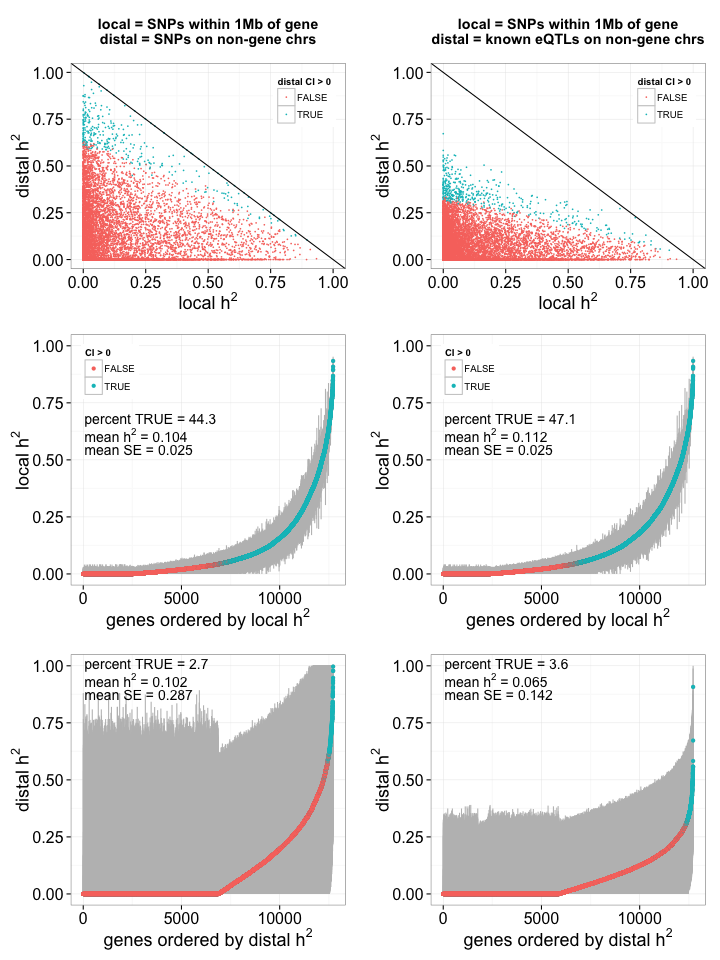
\includegraphics[width=12cm]{Figures/Fig-DGN-jt-h2.png}
\caption{{\bf DGN whole blood expression joint heritability
(h\textsuperscript{2}).} Local (SNPs within 1 Mb of each gene) and distal
(Left: SNPs on non-gene chromsomes. Right: SNPs that are eQTLs in the
Framingham Heart Study on other chromosomes {[}FDR \textless{} 0.05{]})
h\textsuperscript{2} for gene expression were jointly estimated.
(\textbf{Top}) Distal h\textsuperscript{2} compared to local
h\textsuperscript{2} per gene in each model. (\textbf{Middle}) Local and
(\textbf{Bottom}) distal gene expression h\textsuperscript{2} estimates
ordered by increasing h\textsuperscript{2}. The 95\% confidence interval
(CI) of each h\textsuperscript{2} estimate is in gray and genes with a
lower bound greater than zero are in blue.}
\label{fig-dgn-jt-h2}
\end{figure}

Since it has been shown that local-eQTLs are more likely to be distal-eQTLs of target genes, we tested whether restricting the distal genetic similarity computation to QTLs (as determined in the Framingham mRNA dataset of over 5000 individuals \cite{Zhang_2015} \hl{this paper is on isoform QTL I thought. Do they make the cis and trans eQTL results available in this paper? I couldn't find their eQTL paper. We may have to use our own eQTL analysis of Framingham here...} independent of the DGN and GTEx cohorts) for other genes could improve distal heritability precision by prioritizing functional variants. We exclude eQTLs on the same chromosome as the tested gene to avoid contaminating distal h$^2$ with cis associations. 

Using functional priors (known eQTLs) to define distal h\textsuperscript{2} increased the percentage of genes with a positive CI from 2.7\% (343 genes) to 3.6\% (458) in whole blood (Fig. \ref{fig-dgn-jt-h2}). A total of 125 genes have significant distal h$^2$ by both approaches, i.e. all variants on other chromosomes or only  known eQTL variants on other chromosomes.

However, using the subset of known eQTLs (from an independent source) in other chromosomes for computing distal heritability reduced the mean value from 0.102 to 0.065 \hl{wasn't the distal h2 3.4\%?}. Therefore, while we gain some power to detect significant distal heritability by using priors, a good portion of the distal regulation is lost when using only the smaller subset of potentially more functional variants. We used functional priors to estimate distal h$^2$ in the GTEx cohort, but less than 1\% of genes had a positive CI (\nameref{S1_Fig}).

Given the limited sample size we will focus on local regulation for the remainder of the paper.

\subsection*{Sparse local architecture implied by sparsity of best prediction models }\label{the-effect-of-local-genetic-variation-on-gene-expression-is-sparse-rather-than-polygenic}

Next, we sought to determine whether the local genetic contribution to gene expression is polygenic or sparse. In other words, whether many variants with small effects or a small number of large effects were contributing to expression trait variability. For this, we first looked at the prediction performance of a range of models with different degrees of polygenicity, such as the elastic net model with different mixing parameter values that range from 0 (fully polygenic, ridge regression) to 1 (sparse, LASSO).

More specifically, we performed 10-fold cross-validation using the elastic net \cite{Zou_2005} to test the predictive performance of local SNPs for gene expression across a range of mixing parameters ($\alpha$). The mixing parameter that yields the largest cross-validation R\textsuperscript{2} informs the degree of sparsity of each gene expression trait. That is, at one extreme, if the optimal \(\alpha=0\) (equivalent to ridge regression), the gene expression trait is highly polygenic, whereas if the optimal \(\alpha=1\) (equivalent to LASSO), the trait is highly sparse. We found that for most gene expression traits, the cross-validated R\textsuperscript{2} was smaller for \(\alpha=0\) and \(\alpha=0.05\), but nearly identically for \(\alpha=0.5\) through \(\alpha=1\) in the DGN cohort (Fig. \ref{fig-dgn-en}). An \(\alpha=0.05\) was also clearly suboptimal for gene expression prediction in the GTEx tissues, while models with \(\alpha=0.5,0.95,\) or 1 had similar predictive power (\nameref{S2_Fig}). This suggests that for most genes, the effect of local genetic variation on gene expression is sparse rather than polygenic.

\begin{figure}[h]
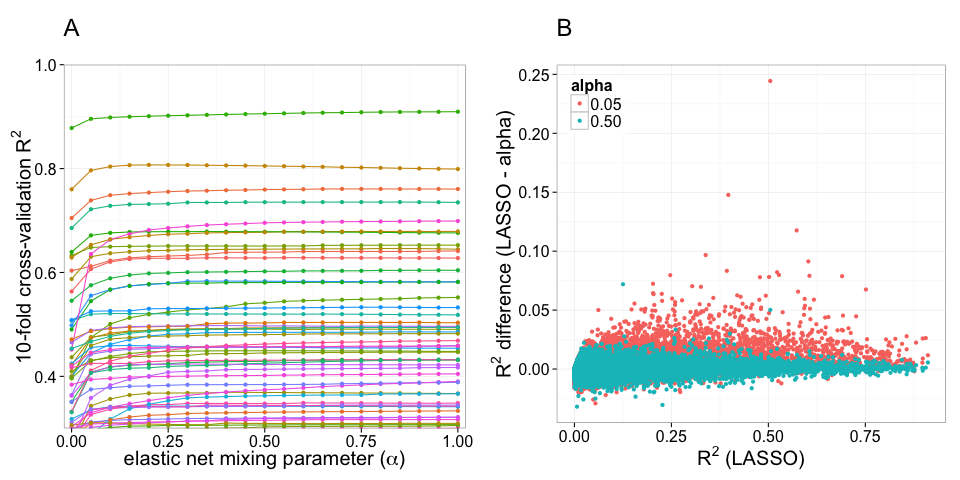
\includegraphics[width=12cm]{Figures/Fig-DGN-EN.png}
\caption{{\bf DGN cross-validated predictive performance across the elastic net.} 
(\textbf{A}) 10-fold cross-validated R\textsuperscript{2} of
predicted vs. observed expression in DGN whole blood compared to a range
of elastic net mixing parameters (\(\alpha\)) for genes on chromosome 22
with R\textsuperscript{2} \textgreater{} 0.3. (\textbf{B}) Predictive
R\textsuperscript{2} difference between LASSO (\(\alpha = 1\)) and
several other values of \(\alpha\) compared to LASSO predictive
R\textsuperscript{2} for all autosomal genes.}
\label{fig-dgn-en}
\end{figure}

\subsection*{Direct estimation of sparsity using BSLMM also points to sparse local architecture}

To further confirm the local sparsity of gene expression traits, we turned to the BSLMM \cite{Zhou_2013} approach, which models the genetic contribution as the sum of a sparse and a polygenic component. The parameter PGE in this model represents the proportion of genetic variance explained by sparse effects. Another parameter, the total variance explained (PVE) by additive genetic variants, is a more flexible Bayesian equivalent of the chip heritability we have estimated using a linear mixed model (LMM) as implemented in GCTA. 

As anticipated, we find that for highly heritable genes, the sparse component is large. For example, all genes with PVE \textgreater{} 0.50 had PGE \textgreater{} 0.82 and their median PGE was 0.989 (Fig. \ref{fig-dgn-bslmm}A). The median PGE for genes with PVE \textgreater{} 0.1 was 0.949. Fittingly, for most (96.3\%) of the genes with PVE estimates \textgreater{} 0.10, the median number of SNPs included in the model was no more than 10 (Fig. \ref{fig-dgn-bslmm}B).

\begin{figure}[h]
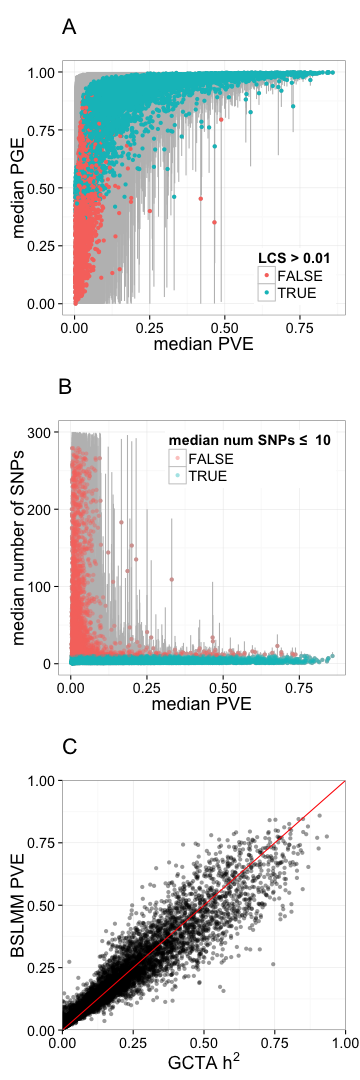
\includegraphics[width=6cm]{Figures/Fig-DGN-BSLMM.png}
\caption{{\bf Bayesian Sparse Linear Mixed Models reveal the sparsity of gene expression architecture.} 
(\textbf{A}) Comparison of median PGE
(proportion of PVE explained by sparse effects) to median PVE (total
proportion of variance explained) for expression of each gene. The 95\%
credible set of each PGE estimate is in gray and genes with a lower
credible set (LCS) greater than 0.01 are in blue. (\textbf{B})
Comparison of the median number of SNPs included in the model of each
gene to median PVE. The 95\% credible set of each SNP-number estimate is
in gray and genes with a median of 10 or fewer SNPs are in blue.(\textbf{C}) 
BSLMM-estimated PVE compared to GCTA-estimated
heritability per gene (R=0.96).}
\label{fig-dgn-bslmm}
\end{figure}

Also as expected, we find that when the sample size is large enough, such as in DGN, there is a strong correlation between BSLMM-estimated PVE and GCTA-estimated h\textsuperscript{2} (Fig. \ref{fig-dgn-bslmm}C, R=0.96). In contrast, when we applied BSLMM to the GTEx data, we found that many genes had strikingly larger BSLMM-estimated PVE than GCTA-estimated h\textsuperscript{2} (Fig. \ref{fig-gtex-pve-h2}). This is further confirmation of the local sparse architecture of gene expression traits: the underlying assumption in the GCTA (LMM) approach to estimate heritability is that the genetic effect sizes are normally distributed, i.e. most variants have small effect sizes. LMM is quite robust to departure from this assumption, but only when the sample size is rather large. For the relatively small sample sizes in GTEx (\(n \leq 361\)), we found that a model that directly addresses the sparse component such as BSLMM outperforms GCTA for estimating h$^2$.

\begin{figure}[h]
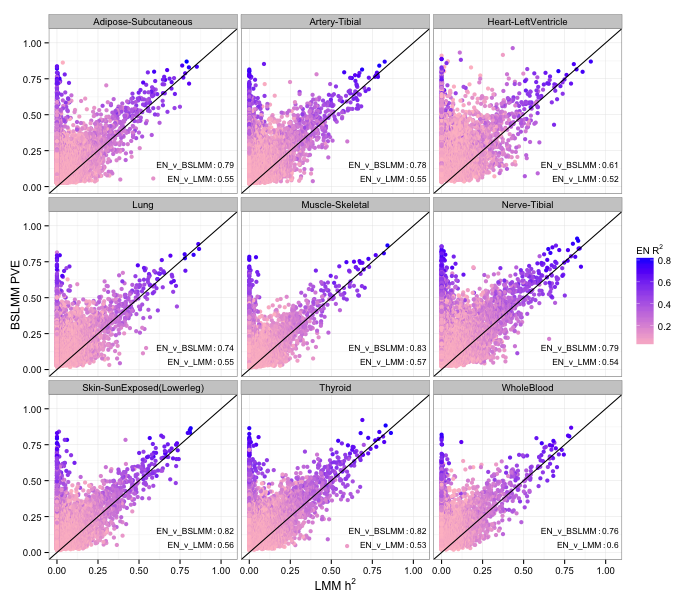
\includegraphics[width=12cm]{Figures/Fig-GTEx_TW_PVE_v_h2.png}
\caption{{\bf GTEx PVE vs. h$^2$.} 
GTEx whole tissue expression BSLMM-estimated PVE (total proportion of variance 
explained) compared to GCTA-estimated heritability per gene. R = Pearson correlation.}
\label{fig-gtex-pve-h2}
\end{figure}

%To further validate this result, we used BSLMM {[}18{]} to
%define the total proportion of variance in expression explained by
%sparse and polygenic effects together (PVE) and the proportion of this
% genetic variance explained by sparse effects (PGE) for local SNPs in
% each gene in the DGN cohort. The PVE can be thought of as a Bayesian
% estimate of chip heritability and, indeed, there is a strong correlation
% between BSLMM-estimated PVE and GCTA-estimated h\textsuperscript{2} (Fig
% 6A, R=0.96). For genes with large PVE, the PGE also was large,
% indicative of a sparse genetic architecture. For example, all genes with
% PVE \textgreater{} 0.50 had PGE \textgreater{} 0.82 and their median PGE
% was 0.989 (Fig 6B). The median PGE for genes with PVE \textgreater{} 0.1
% was 0.949. Fittingly, for most (96.3\%) of the genes with PVE estimates
% \textgreater{} 0.10, the median number of SNPs included in the model was
% no more than 10 (Fig 6C).

% This likely reflects the increased power
% of the BSLMM method at the lower sample sizes  present
% in GTEx to estimate variance explained when the trait is more sparse
% than polygenic. GCTA assumes an underlying polygenic model, but as we
% saw in DGN, BSLMM-estimated PVE and GCTA-estimated h\textsuperscript{2}
% are more correlated when the sample size is larger (n=922, Fig 6A). As
% we observed in DGN, genes with larger PVE estimates were more likely to
% have a PGE estimate approaching 1 with a lower credible set greater than
% 0.01 in each of the nine GTEx tissues (Fig 8).

\subsection*{Orthogonal decomposition of cross-tissue and tissue-specific expression traits}

Since a substantial portion of local regulation was shown to be common across multiple tissues \cite{Ardlie_2015}, we sought to decompose the expression levels into a component that is common across all tissues and tissue-specific components. For this we use a linear mixed effects model as described in the Methods section. We call this approach orthogonal tissue decomposition (OTD) because the cross-tissue and tissue-specific components are assumed to be independent in the model. The decomposition is applied at the expression trait level so that the downstream genetic regulation analysis is performed separately for each derived trait, cross-tissue and tissue-specific expression, which greatly reduces computational burden. 

\subsection*{Cross-tissue expression phenotype has increased predictive
power}%\label{cross-tissue-expression-phenotype-has-increased-predictive-power-and-recapitulates-known-multi-tissue-eqtl-target-genes}

% Using a marginal
% model with just the local GRM, we estimated the local
% h\textsuperscript{2} of cross-tissue gene expression and tissue-specific
% gene expression in the nine tissues with the most samples.

A clear benefit of OTD for the cross-tissue trait is that the effective sample size of the trait is 450 even though each of the tissues had less than 362 individuals. This is reflected in more precise estimates of h$^2$ as shown below.

For all the derived phenotypes, one cross-tissue and 40 tissue-specific ones, we computed the local heritability and generated prediction models.

The cross-tissue heritability estimates were larger and the standard errors were smaller than the tissue-specific estimates reflecting the fact that a substantial portion of regulation is common across tissues (\nameref{S3_Fig}). The percentage of GCTA h\textsuperscript{2} estimates with positive CIs was much larger for cross-tissue expression (19.8\%) than the tissue-specific expressions (all less than 4\%, \nameref{S1_Table}). Similarly, the percentage of BSLMM PVE estimates with a lower credible set greater than 0.01 was 49\% for cross-tissue expression, but ranged from 24-27\% for tissue-specific expression (\nameref{S4_Fig}).

We also compared the cross-tissue h\textsuperscript{2} from the OTD to h\textsuperscript{2} estimates from the pre-OTD measures of gene expression, which we term whole tissue expression. Again, the cross-tissue heritability estimates were larger and the standard errors were smaller than the whole tissue estimates (\nameref{S5_Fig}) due to the larger effective sample size of the cross tissue phenotypes compared to whole tissue expression phenotypes as well as the common regulation across tissues. The percentage of whole tissue h\textsuperscript{2} estimates with positive CIs ranged from 2.4-9.5\% and were all larger than their respective tissue-specific positive CI percentages, but smaller than the cross-tissue percentage (Table \ref{table-h2}, \nameref{S1_Table}). Cross-tissue BSLMM PVE estimates had lower error than whole tissue PVE (\nameref{S4_Fig}, \nameref{S6_Fig}). Cross-tissue predictive performance exceeded that of both tissue-specific and whole tissue expression as indicated by higher cross-validated R\textsuperscript{2} (\nameref{S2_Fig}, \nameref{S7_Fig}).

Like whole tissue expression, cross-tissue and tissue-specific expression showed better predictive performance when using more sparse models. In other words elastic-net models with \(\alpha \geq 0.5\) predicted better than the ones with \(\alpha=0.05\) (\nameref{S7_Fig}). 


\subsection*{OTD derived phenotypes recapitulate published multi-tissue eQTL results}
%% from README: correspond to the marginal posterior of the SNP being active in Adipose, etc. These columns are the same as in the file "res_final_uc_com_genes_com_snps.txt.gz" (described above), which only contains the best SNP per gene

%\hl{did you download the top eQTL's prob of being eqtl in the tissue? From what I talked with Matthew Stephens I thought it was the probability at the gene level, of the gene being an egene, i.e. being regulated in the tissue by some eqtl.} 
%To Haky, the SNP seems to be the same for each gene. From the README file: "These values may be interpreted as Pr(SNP is eQTL in tissue s | data). 9875 eGenes are presented, with the?top" (most significant) SNP in each gene used."
%first few rows of file res_final_uc_com_genes_com_snps.txt.gz:
%gene	snp	Adipose	Artery	Blood	Heart	Lung	Muscle	Nerve	Skin	Thyroid
%ENSG00000137288.4	rs11759971	0.6596	0.6547	0.5383	0.6264	0.6759	0.5699	0.6750	0.7638	0.6775
%ENSG00000168005.4	rs36077346	0.7835	0.7817	0.7632	0.7743	0.7928	0.5103	0.7922	0.7837	0.7932
%ENSG00000255893.1	rs657249	1.0000	1.0000	0.3647	1.0000	1.0000	1.0000	1.0000	1.0000	1.0000

We compared our OTD results to those from a joint multi-tissue eQTL analysis method \cite{Flutre_2013}, which was previously performed on a subset of the GTEx data \cite{Ardlie_2015}. The results of this analysis include eQTL posterior probabilities for nine tissues, which can be interpreted as the probability a SNP is an eQTL in tissue \emph{x} given the data. Using the top eQTL for each gene, we defined an entropy statistic (see Methods) that combines the nine posterior probabilities into one value such that higher entropy values mean the gene regulation is more uniform across all nine tissues, rather than in just a subset of the nine. We observed a strong correlation between entropy and both the cross-tissue expression heritability (R = 0.082, Fig. \ref{fig-ct-entropy}A) and PVE (R = 0.12, Fig. \ref{fig-ct-entropy}B) estimates, using the cross-tissue expression derived from the OTD. Thus, genes with high cross-tissue heritability are more likely to have cross-tissue eQTLs, confirming that OTD is capturing the cross-tissue component of gene expression. Also, the correlation between tissue-specific OTD gene expression PVE and the posterior probability that the gene has an eQTL in that tissue is strongest in each respective tissue, confirming that OTD also captures tissue-specific components of gene expression (Fig. \ref{fig-corrplot}).

\begin{figure}[h]
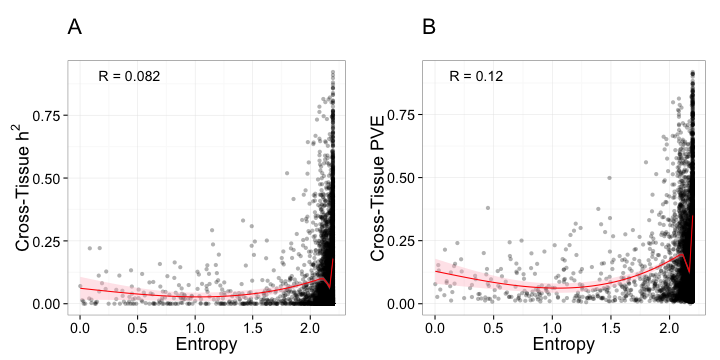
\includegraphics[width=12cm]{Figures/Fig-CT-entropy.png}
\caption{{\bf Cross-tissue expression from the 
orthogonal tissue decomposition (OTD) compared to multi-tissue eQTL results.} 
Pearson correlation (R) between the entropy of the posterior probabilities
from the Flutre et al. multi-tissue eQTL method 
and the estimates of (A) heritability and (B) PVE of cross-tissue
gene expression derived from the OTD. The generalized additive model smoothing 
line is in red.}
\label{fig-ct-entropy}
\end{figure}

\begin{figure}[h]
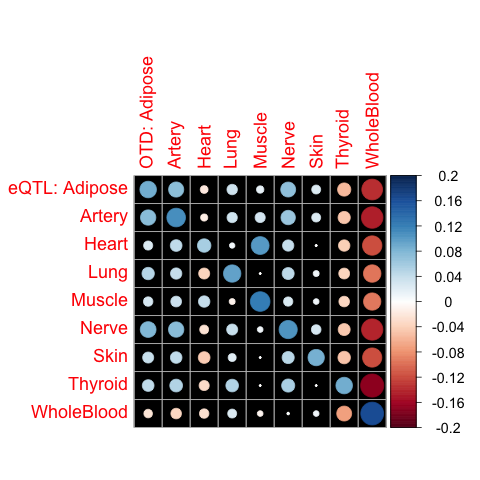
\includegraphics[width=10cm]{Figures/Fig-cor-StephensPr-OTDtsPVE.png}
\caption{{\bf Tissue-specific expression from the 
orthogonal tissue decomposition (OTD) compared to multi-tissue eQTL results.} 
Pearson correlation (R) between the 
posterior probability the top multi-tissue eQTL regulates its gene in a given tissue (eQTL, 
Flutre et al. method) and the PVE of tissue-specific gene expression from the orthogonal
tissue decomposition (OTD). Area of each circle is proportional to the absolute value of R.}
\label{fig-corrplot}
\end{figure}


% Please do not create a heading level below \subsection. For 3rd level headings, use \paragraph{}. 

\section*{Discussion}
Motivated by the key role that regulatory variation plays in the genetic control of complex traits \cite{Nicolae_2010,Nica_2010,Gusev_2014}, we performed a survey of the heritability and patterns of effect sizes of gene expression traits across a comprehensive set of human tissues. We quantified the local and distal heritability of gene expression in DGN and 40 different tissues from the GTEx consortium. For the DGN dataset, we estimate the relative proportion of mean local and distal genetic contribution to gene expression traits. For GTEx samples it was not possible to estimate the mean distal heritability because of the limited sample size. As the number of GTEx samples grows to near 1000 individuals, we expect to be able to estimate these values.

In DGN (whole blood), the mean local h$^2$ was 14.3\% and the mean distal h$^2$ was 3.4\% such that the local variation contribution is estimated as 14.3/(3.4+14.3) = 81\%. This is much higher than the 37\% reported by Price et al. \cite{Price_2011} based on blood expression data from a cohort of Icelandic individuals. This potentially underestimation of the distal component could be due to over-correction of confounders used in the preprocessing of the expression trait data we used. Indeed, PEER \cite{Stegle_2012}, SVA \cite{Leek_2007}, and other types of hidden confounder corrections have been shown to increase local eQTL replicability, but their consequences on distal regulation is not well understood.  As larger sample sizes become available, we will test this hypothesis in GTEx data by computing the distal h$^2$ without PEER factor correction.

%\hl{we need to check whether Battle et al computed the proportion of local vs distal for DGN}
%To Haky, I did not see mention of distal proportion, I did see:
% "...with cis-eQTLs explaining a median of 3.3% of expression variance (median 7.7% among genes with an eQTL),..."

We showed that restricting distal variants to known functional variants such as eQTL data from independent studies improves the precision of distal heritability estimates, but also reduces mean distal heritability estimates by half. For GTEx tissues, we computed the distal heritability using only the subset of functional (known eQTLs) variants to reduce the errors in the estimates at the expense of missing variants that contribute to the traits.

Using results implied by the improved predictive performance of sparse models and by directly estimating sparsity using BSLMM (Bayesian Sparse Linear Mixed Model), we show evidence that for highly heritable genes, local regulation is sparse across all the tissues analyzed here. For genes with moderate and low heritability the evidence is not as strong, but results are consistent with a sparse local architecture. Better methods to correct for hidden confounders that do not dilute distal signals and larger sample sizes will be needed to determine the properties of distal regulation. 

Given that a substantial portion of local regulation is shared across tissues, we propose here to decompose the expression traits into cross-tissue and tissue-specific components. This approach, called orthogonal tissue decomposition, aims to decouple the shared regulation from the tissue-specific regulation. We examined the genetic architecture of these derived traits and find that they follow similar patterns to the original whole tissue expression traits. The cross-tissue component benefits from an effectively larger sample size than any individual tissue trait, which is reflected in more accurate heritability estimates and consistently better prediction performance. Encouragingly, heritability estimates of cross-tissue traits correlate well with a measure of uniformity of regulation across tissues defined as the entropy of the vector of probability for a gene to be regulated in a given tissue. Higher entropy genes will show more uniform regulation across tissues. As for the tissue-specific expression traits, we found that they recapitulate correlation with the vector of probability of tissue-specific regulation. The main application for which these traits were devised is to be used as prediction models in PrediXcan \cite{Gamazon_2015}. We expect results from the cross-tissue models to relate to mechanisms that are shared across multiple tissues whereas results from the tissue-specific models will inform us about the context specific mechanisms. 

% In DGN, the mean local
% h\textsuperscript{2} was 0.13, similar to that found in family studies
% of blood expression, where mean h\textsuperscript{2} ranged from
% 0.07-0.11 {[}11,12{]}. While we found that functional priors (known
% trans-eQTLs) can reduce the error of the estimate by reducing the number
% of genetic markers included in the genetic relationship matrix, larger
% sample sizes (n \textgreater{} 1000) are needed to accurately estimate
% distal heritability.

% Using the hybrid polygenic-sparse approach of BSLMM (Bayesian Sparse
% Linear Mixed Model) {[}18{]}, we show that the local architecture of
% gene expression is sparse (high PGE) for most heritable genes in both
% DGN and GTEx. Using the elastic net {[}24{]}, we observed improved
% cross-validated expression prediction for \(\alpha \geq 0.5\) across
% tissues, confirming the sparsity result. This result demonstrates that
% sparse effects can be identified with sample sizes in the hundreds
% rather than the thousands and is supported by many prior studies with
% sample sizes near 100 that identified replicable eQTLs near the
% transcription start sites of genes{[}9{]}. Conversely, for traits that
% are highly polygenic, e.g.~height, BMI, schizophrenia, and bipolar
% disorder, thousands to tens of thousands of samples are needed to
% identify significant genetic signals {[}26{]}. Therefore, the distal
% contributions to expression h\textsuperscript{2} are thought to be more
% polygenic because they could not be accurately estimated here with
% sample sizes in the hundreds. \hl{not exactly}
%
% Our BSLMM analysis quantified the optimal number of SNPs to include for
% each gene. For example, the median number of SNPs for \emph{ERAP2} was
% 1. When we previously plotted out-of-sample observed vs.~predicted
% expression using elastic net (\(\alpha=0.5\)) generated predictors for
% this gene, we saw three clusters, corresponding to each of the three
% genotypes for the causal variant {[}13{]}. Similarly, BSLMM estimated 2,
% 3, and 5 SNPs for \emph{PEX6}, \emph{NUDT2}, and \emph{ERAP1},
% respectively, consistent with the out-of-sample observed vs.~predicted
% expression plots in our PrediXcan paper (see Figure 5 in {[}13{]}).
% Potentially due to variations in imputation quality of the input SNPs
% for expression prediction, it is useful to include more than the likely
% causal variants (i.e.~elastic net rather than BSLMM) in the prediction
% for robustness. In addition, the elastic net is amenable
% cross-validation, while genome-wide cross-validation with BSLMM is
% impractical at current runtimes.
%
% We developed a mixed effects model called orthogonal tissue
% decomposition (OTD) to determine the cross-tissue and tissue-specific
% components of gene expression in the GTEx dataset. Previous studys have
% shown that many eQTLs are shared across tissues {[}21,25{]}. In
% addition, because expression data from multiple tissues were available
% from the same individuals in GTEx, we could effectively use the multiple
% tissue samples as subject replicates in our OTD model. However, the
% tissue availability is unbalanced across individuals because of the
% difficulties of sample collection and the uneven quality of the tissues.
% By combining all available expression data in our OTD model, we found
% that estimates of the local heritability of cross-tissue gene expression
% have larger magnitude and improved standard errors compared to single
% tissue estimates due to the borrowing of information across all samples.
% Thus, OTD effectively increases power to estimate heritability.
% Comparing our OTD results to a previously performed joint multi-tissue
% eQTL analysis method {[}25{]}, we show that genes with high cross-tissue
% heritability are more likely to have cross-tissue eQTLs, confirming that
% OTD is capturing the cross-tissue component of gene expression.
%
% We confirmed that OTD also captures tissue-specific components of gene
% expression by showing the correlation between tissue-specific OTD gene
% expression PVE and the posterior probability that the gene has an eQTL
% in that tissue is strongest in each respective tissue. Interestingly,
% whole blood and thyroid appear to be outliers in that they each have a
% negative correlation with all the other tissues (Fig 15). In the GTEx
% pilot analysis, whole blood had the lowest levels of eQTL sharing with
% other tissues and thyroid had the largest number of cis-eQTL genes,
% which implies a higher number of tissue-specific eQTLs {[}21{]}.

In this paper, we quantitate the genetic architecture of gene expression and develop predictors across tissues. We show that local heritability can be accurately estimated across tissues, but distal heritability cannot be reliably estimated at current sample sizes. Using two different approaches, the elastic net and BSLMM, we show that for local gene regulation, the genetic architecture is mostly sparse rather than polygenic. Using new expression phenotypes generated in our OTD model, we show that cross-tissue predictive performance exceeded that of both tissue-specific and whole tissue expression as indicated by higher elastic net cross-validated R\textsuperscript{2}. Predictors generated in this study of gene expression architecture have been added to our PredictDB database (\url{https://github.com/hakyimlab/PrediXcan}) for use in future studies of complex trait genetics.


% You may title this section "Methods" or "Models". 
% "Models" is not a valid title for PLoS ONE authors. However, PLoS ONE
% authors may use "Analysis" 
\section*{Materials and Methods}
\subsection*{Genomic and Transcriptomic
Data}\label{genomic-and-transcriptomic-data}

\paragraph*{DGN Dataset.}\label{dgn-dataset}

We obtained whole blood RNA-seq and genome-wide genotype data for 922
individuals from the Depression Genes and Networks (DGN) cohort
\cite{Battle_2013}, all of European ancestry. For our analyses, we used the HCP
(hidden covariates with prior) normalized gene-level expression data
used for the \emph{trans}-eQTL analysis in Battle et al. \cite{Battle_2013} and
downloaded from the NIMH repository. The 922 individuals were unrelated
(all pairwise \(\hat{\pi}\) \textless{} 0.05) and thus all included in
downstream analyses. Imputation of approximately 650K input SNPs (minor
allele frequency {[}MAF{]} \textgreater{} 0.05, Hardy-Weinberg
Equilibrium {[}P \textgreater{} 0.05{]}, non-ambiguous strand {[}no A/T
or C/G SNPs{]}) was performed on the University of Michigan
Imputation-Server
(\url{https://imputationserver.sph.umich.edu/start.html}) \cite{Howie_2012,Fuchsberger_2014}
with the following parameters: 1000G Phase 1 v3 ShapeIt2 (no singletons)
reference panel, SHAPEIT phasing, and EUR population. Approximately 1.9M
non-ambiguous strand SNPs with MAF \textgreater{} 0.05, imputation
R\textsuperscript{2} \textgreater{} 0.8 and, to reduce computational
burden, inclusion in HapMap Phase II were retained for subsequent
analyses.

\paragraph*{GTEx Dataset.}\label{gtex-dataset}

We obtained RNA-seq gene expression levels from 8555 tissue samples (53
unique tissue types) from 544 unique subjects in the GTEx Project \cite{Ardlie_2015} 
data release on 2014-06-13. Of the individuals with gene
expression data, genome-wide genotypes (imputed with 1000 Genomes) were
available for 450 individuals. While all 8555 tissue samples were used
in the OTD model (described below) to generate cross-tissue and
tissue-specific components of gene expression, we used the 40 tissues
with the largest sample sizes when quantifying tissue-specific effects (see Table \ref{table-h2}).
Approximately 2.6M non-ambiguous strand SNPs included in HapMap Phase II were retained for
subsequent analyses.

\subsection*{Partitioning local and distal heritability of gene
expression}\label{partitioning-local-and-distal-heritability-of-gene-expression}

Motivated by the observed differences in regulatory effect sizes of variants located in the vicinity of the genes and distal to the gene,
we partitioned the proportion of gene expression variance explained by
SNPs in the DGN cohort into two components: local (SNPs within 1Mb of
the gene) and distal (eQTLs on non-gene chromosomes) as defined by the
GENCODE \cite{Harrow_2012} version 12 gene annotation. We calculated the
proportion of the variance (narrow-sense heritability) explained by each
component using the following mixed-effects model:

\[ Y_g = \sum_{k  \in local}w_{k,g} X_k + \sum_{k  \in distal}w_{k,g} X_k + \epsilon \]

Assuming a random effects for \(w_{k,g} \sim N(0, \sigma^2_w)\) and
\(\epsilon \sim N(0, \sigma^2_{\epsilon} I_n)\), where \(I_n\) is the
identity matrix, we calculated the total variability explained by local
and distal components by estimating \(\sigma^2_w\) with restricted
maximum likelihood (REML) using GCTA software \cite{Yang_2011}. For heritability
analyses in the GTEx cohort, we removed the \(distal\) term from the
model and only estimated marginal \(local\) h\textsuperscript{2} due to
the smaller sample sizes of both cross-tissue and tissue-specific
expression levels compared to DGN. 

Approximate confidence intervals were computed as the point estimate $\pm$ 
2 times the estimated standard error. The intervals were also forced to be $\ge 0 $ or $\le 1$. 
Genes were considered to have heritability significantly different from 0 if the confidence interval did not include 0.

By default we restricted the heritability estimates to be in the 0 to 1 interval. However, 
for the purpose of estimating the mean heritability (see Table \ref{table-h2} and \nameref{S1_Table}), we performed separate runs allowing the heritability estimates to 
take negative values with the \texttt{--reml-no-constrain} option in GCTA. Despite the lack of obvious biological interpretation of a negative heritability, 
it is an accepted procedure used in order to avoid bias in the estimated mean \cite{Price_2011,Wright_2014}.

\subsection*{Determining polygenicity versus sparsity using the elastic
net}\label{determining-polygenicity-versus-sparsity-using-the-elastic-net}

We used the glmnet package to fit an elastic net model where the tuning parameter is chosen via 10 fold cross validation to maximize prediction performance measure by Pearson's R$^2$ \cite{Friedman_2010, Simon_2011}.

%  applied the elastic net {[}24{]} to model the effect of local genetic
% variation (SNPs within 1 Mb of gene) on the genetic architecture of gene
% expression. We used the \texttt{cv.glmnet} function in the R package
% \texttt{glmnet} {[}30,31{]} to perform 10-fold cross-validation of the
% elastic net across a range of tuning paramaters (\(\lambda\)) to find the
% one that maximized predictive performance, measured by Pearson's
% R\textsuperscript{2}.
% over a grid of values of \(\lambda\) covering the entire range
% {[}30,31{]}. This tuning parameter \(\lambda\) controls the overall
% strength of the penalty.

The elastic net penalty is controlled by mixing parameter \(\alpha\),
which spans LASSO (\(\alpha=1\), the default) \cite{Tibshirani_1996} at one extreme
and ridge regression (\(\alpha=0\)) \cite{Hoerl_1970} at the other. The ridge
penalty shrinks the coefficients of correlated SNPs towards each other,
while the LASSO tends to pick one of the correlated SNPs and discard the
others. Thus, an optimal prediction R\textsuperscript{2} for
\(\alpha=0\) means the gene expression trait is highly polygenic, while
an optimal prediction R\textsuperscript{2} for \(\alpha=1\) means the
trait is highly sparse. 

In the DGN cohort, we tested 21 values of the mixing parameter
(\(\alpha=0, 0.05, 0.1, ..., 0.90, 0.95, 1\)) for optimal prediction of
gene expression of the 341 genes on chromosome 22. For the rest of the
autosomes in DGN and for whole tissue, cross-tissue, and tissue-specific
expression in the GTEx cohort, we tested \(\alpha=0.05, 0.5, 0.95, 1\).

\subsection*{Quantifying sparsity with Bayesian Sparse Linear Mixed
Models
(BSLMM)}\label{quantifying-sparsity-with-bayesian-sparse-linear-mixed-models-bslmm}

We used BSLMM \cite{Zhou_2013} to model the effect of local genetic variation
(SNPs within 1 Mb of gene) on the genetic architecture of gene
expression. The BSLMM is a linear model with a polygenic component (small effects) and a sparse component (large effects)
enforced by sparsity inducing priors on the
regression coefficients \cite{Zhou_2013}. We used the software GEMMA \cite{Zhou_2012} to
implement BSLMM for each gene using the following parameters:

\[ \texttt{gemma -g [genoFile] -p [expFile] -a [snpFile] -bslmm 1 -s 100000 -o [out]} \]

The \texttt{-bslmm 1} option specifies a linear BSLMM and the
\texttt{-s 100000} option specifies the number of sampling steps per
gene. The BSLMM estimates the PVE (the total proportion of variance in
phenotype explained by the sparse effects and random effects terms
together) and PGE (the proportion of genetic variance explained by the
sparse effects terms). From the second half of the sampling iterations
for each gene, we report the median and the 95\% credible sets of the
PVE, PGE, and the \textbar{}\(\gamma\)\textbar{} parameter (the number
of SNPs with non-zero coefficients).

\subsection*{Orthogonal tissue
decomposition}\label{orthogonal-tissue-decomposition}

To better understand the context specificity of gene expression
regulation, we developed a method called orthogonal tissue decomposition
(OTD). This approach is an extension of our method to develop an
intrinsic growth phenotype \cite{Im_2012}. We applied OTD to GTEx Project
\cite{Ardlie_2015} data and decomposed the expression of each gene into
cross-tissue and tissue-specific components. The tissue availability is
unbalanced across individuals because of the difficulties of sample
collection and the uneven quality of the tissues. OTD decomposes the
expression traits into orthogonal components as represented by the
following model:

\[ Y_i = T_{i,cross} + T_{i,tissue} \]

Specifically, to generate cross-tissue and tissue-specific expression
levels, we used the \texttt{lmer} function in the R \cite{R_Core_Team_2015} package
\texttt{lme4} \cite{Bates_2015a} to fit the following mixed-effects model:

\[ \texttt{fit <- lme4::lmer(expression $\sim$ (1|SUBJID) + TISSUE + GENDER + PEERs)} \]

The model included whole tissue gene expression levels in 8555 GTEx
tissue samples from 544 unique subjects. A total of 17,647
Protein-coding genes (defined by GENCODE \cite{Harrow_2012} version 18) with a
mean gene expression level across tissues greater than 0.1 RPKM (reads
per kilobase of transcript per million reads mapped) and RPKM $>$ 0 in at least 3 individuals were included in
the model. \texttt{SUBJID} was a random effect and the covariates
\texttt{TISSUE}, \texttt{GENDER}, and \texttt{PEERs} were fixed effects
used to predict whole tissue expression levels (\texttt{expression} in
the model). \texttt{PEERs} included the top 15 PEER factors estimated
across all tissues using the R package \texttt{PEER} \cite{Stegle_2012} to control
for batch effects and experimental confounders. Cross-tissue expression
was defined as the random effects from the model (\texttt{ranef(fit)})
and tissue-specific expression as the residuals (\texttt{resid(fit})).

\subsection*{Comparison of OTD PVE to multi-tissue eQTL
results}\label{comparison-of-otd-pve-to-multi-tissue-eqtl-results}

Using results from a joint multi-tissue eQTL analysis method \cite{Flutre_2013}
performed with a subset of the GTEx data (maximum n=175 in the nine
tissues of the pilot phase, see \cite{Ardlie_2015}), we defined an entropy
statistic to compare these results to those from our OTD method. The
results of the multi-tissue analysis include eQTL posterior
probabilities for each of the nine tissues, which can be interpreted as
the probability a SNP is an eQTL in tissue \(t\) given the data. Using
the top eQTL for each gene \(g\), we defined the entropy \(S_g\) as:

\[ S_g = -\sum_{t}p_{t,g} \log p_{t,g} \]

where \(p_{t,g}\) is the eQTL probability in tissue \(t\) normalized to
1 for each gene \(g\). Thus, eQTLs with higher entropy statistics are
more likely to be cross-tissue eQTLs, rather than only regulating gene
expression in one or a few tissues. We calculated the Pearson
correlation between \(S_g\) and the cross-tissue expression heritability
and PVE for each gene to verify that our OTD method captures
cross-tissue effects. We also calculated a Pearson correlation matrix
between the posterior probabilities in each tissue from the multi-tissue
eQTL method and the tissue-specific gene expression PVE from the OTD
method.



\section*{Acknowledgments}
We thank Nicholas Knoblauch and Jason Torres for initial pipeline
development and planning.

\subsection*{Grants}\label{grants}

We acknowledge the following US National Institutes of Health grants:
R01MH107666 (H.K.I.), K12 CA139160 (H.K.I.), T32 MH020065 (K.P.S.), R01 MH101820 (GTEx), 
P30 DK20595 and P60 DK20595 (Diabetes Research and
Training Center), P50 DA037844 (Rat Genomics), P50 MH094267 (Conte). H.E.W. was
supported in part by start-up funds from Loyola University Chicago.


\paragraph{GTEx data.}\label{gtex-data}

The Genotype-Tissue Expression (GTEx) Project was supported by the
Common Fund of the Office of the Director of the National Institutes of
Health (commonfund.nih.gov/GTEx). Additional funds were provided by the
NCI, NHGRI, NHLBI, NIDA, NIMH, and NINDS. Donors were enrolled at
Biospecimen Source Sites funded by NCI Leidos Biomedical Research, Inc.
subcontracts to the National Disease Research Interchange (10XS170),
Roswell Park Cancer Institute (10XS171), and Science Care, Inc.
(X10S172). The Laboratory, Data Analysis, and Coordinating Center
(LDACC) was funded through a contract (HHSN268201000029C) to the The
Broad Institute, Inc. Biorepository operations were funded through a
Leidos Biomedical Research, Inc. subcontract to Van Andel Research
Institute (10ST1035). Additional data repository and project management
were provided by Leidos Biomedical Research, Inc.(HHSN261200800001E).
The Brain Bank was supported supplements to University of Miami grant
DA006227. Statistical Methods development grants were made to the
University of Geneva (MH090941 \& MH101814), the University of Chicago
(MH090951,MH090937, MH101825, \& MH101820), the University of North
Carolina - Chapel Hill (MH090936), North Carolina State University
(MH101819),Harvard University (MH090948), Stanford University
(MH101782), Washington University (MH101810), and to the University of
Pennsylvania (MH101822). The datasets used for the analyses described in
this manuscript were obtained from dbGaP at
\url{http://www.ncbi.nlm.nih.gov/gap} through dbGaP accession number
phs000424.v3.p1.

\paragraph{DGN data.}\label{dgn-data}

NIMH Study 7 (GenRED I) - Data and biomaterials were collected in six
projects that participated in the National Institute of Mental Health
(NIMH) Genetics of Recurrent Early-Onset Depression (GenRED) project.
From 1999-2003, the Principal Investigators and Co-Investigators were:
New York State Psychiatric Institute, New York, NY, R01 MH060912, Myrna
M. Weissman, Ph.D.~and James K. Knowles, M.D., Ph.D.; University of
Pittsburgh, Pittsburgh, PA, R01 MH060866, George S. Zubenko, M.D.,
Ph.D.~and Wendy N. Zubenko, Ed.D., R.N., C.S.; Johns Hopkins University,
Baltimore, MD, R01 MH059552, J. Raymond DePaulo, M.D., Melvin G.
McInnis, M.D.~and Dean MacKinnon, M.D.; University of Pennsylvania,
Philadelphia, PA, RO1 MH61686, Douglas F. Levinson, M.D. (GenRED
coordinator), Madeleine M. Gladis, Ph.D., Kathleen MurphyEberenz,
Ph.D.~and Peter Holmans, Ph.D. (University of Wales College of
Medicine); this preprint is the author/funder. It is made available
under a CC-BY 4.0 International license. bioRxiv preprint first posted
online June 17, 2015; doi: \url{http://dx.doi.org/10.1101/020164}; The
copyright holder for University of Iowa, Iowa City, IW, R01 MH059542,
Raymond R. Crowe, M.D.~and William H. Coryell, M.D.; Rush University
Medical Center, Chicago, IL, R01 MH059541- 05, William A. Scheftner,
M.D., Rush-Presbyterian. NIMH Study 18 - Data and biomaterials were
obtained from the limited access datasets distributed from the
NIH-supported ``Sequenced Treatment Alternatives to Relieve Depression''
(STAR*D). STAR*D focused on non-psychotic major depressive disorder in
adults seen in outpatient settings. The primary purpose of this research
study was to determine which treatments work best if the first treatment
with medication does not produce an acceptable response. The study was
supported by NIMH Contract \# N01MH90003 to the University of Texas
Southwestern Medical Center. The ClinicalTrials.gov identifier is
NCT00021528. NIMH Study 52 (GenRED II) -- Data and biomaterials in this
release were collected in six projects that participated in the National
Institute of Mental Health (NIMH) Genetics of Recurrent Early-Onset
Depression (GenRED) project (1999-2009). The Principal Investigators and
Co-Investigators were: New York State Psychiatric Institute, New York,
NY, R01 MH 060912, Myrna M. Weissman, Ph.D.; Johns Hopkins University,
Baltimore, MD, R01 MH059552, J. Raymond DePaulo, M.D., and James B.
Potash, M.D., M.P.H.; University of Pennsylvania, Philadelphia, PA
(1999-2005), and Stanford University (2006-2009), R01 MH61686, Douglas
F. Levinson, M.D. (GenRED coordinator); University of Iowa, Iowa City,
IW, R01 MH059542e, Raymond R. Crowe, M.D., and William H. Coryell, M.D.;
Rush University Medical Center, Chicago, IL, R01 MH059541-05, William A.
Scheftner, M.D.; and University of Pittsburgh, Pittsburgh, PA
(1999-2003), R01 MH060866, George S. Zubenko, M.D., Ph.D., and Wendy N.
Zubenko, Ed.D., R.N., C.S. NIMH Study 88 -- Data was provided by
Dr.~Douglas F. Levinson. We gratefully acknowledge the resources were
supported by National Institutes of Health/National Institute of Mental
Health grants 5RC2MH089916 (PI: Douglas F. Levinson, M.D.;
Coinvestigators: Myrna M. Weissman, Ph.D., James B. Potash, M.D., MPH,
Daphne Koller, Ph.D., and Alexander E. Urban, Ph.D.) and 3R01MH090941
(Co-investigator: Daphne Koller, Ph.D.).

\paragraph{Computing resources.}\label{computing-resources}

This work made use of the Open Science Data Cloud (OSDC) which is an
Open Cloud Consortium (OCC)-sponsored project. This work was supported
in part by grants from Gordon and Betty Moore Foundation and the
National Science Foundation and major contributions from OCC members
like the University of Chicago. this preprint is the author/funder. It
is made available under a CC-BY 4.0 International license. bioRxiv
preprint first posted online June 17, 2015; doi:
\url{http://dx.doi.org/10.1101/020164}; The copyright holder for
\url{https://www.opensciencedatacloud.org/} Grossman RL, Greenway M,
Heath AP, Powell R, Suarez R, Wells W, White KP, Atkinson M, Klampanos
I, Alvarez H, Harvey C and Mambretti J, The Design of a Community
Science Cloud: The Open Science Data Cloud Perspective. (2012)
\url{doi:10.1109/SC.Companion.2012.127} This work made use of the
Bionimbus Protected Data Cloud (PDC), which is a collaboration between
the Open Science Data Cloud (OSDC) and the IGSB (IGSB), the Center for
Research Informatics (CRI), the Institute for Translational Medicine
(ITM), and the University of Chicago Comprehensive Cancer Center
(UCCCC). The Bionimbus PDC is part of the OSDC ecosystem and is funded
as a pilot project by the NIH.
\url{https://www.bionimbus-pdc.opensciencedatacloud.org/} Heath AP,
Greenway M, Powell R, Spring J, Suarez R, Hanley D, Bandlamudi C,
McNerney ME, White KP and Grossman RL, Bionimbus: A Cloud for Managing,
Analyzing and Sharing Large Genomics Datasets. J Am Med Inform Assoc
(2014) \url{doi:10.1136/amiajnl-2013-002155}


\nolinenumbers


% Either type in your references using
% \begin{thebibliography}{}
% \bibitem{}
% Text
% \end{thebibliography}
%
% OR
%
% Compile your BiBTeX database using our plos2015.bst
% style file and paste the contents of your .bbl file
% here.
% 

\bibliography{GenArch_references}

\section*{Supporting Information}

% Include only the SI item label in the subsection heading. Use the \nameref{label} command to cite SI items in the text.

\subsection*{S1 Fig}
%Fig-GTEx_TW_glo.jt.h2.tiff
\label{S1_Fig}
{\bf GTEx whole tissue distal heritability (h$^2$) estimation.} Distal (SNPs that are eQTLs in the Framingham Heart Study on other chromosomes [FDR $<$ 0.05]) gene expression h$^2$ estimates from a joint model in the nine GTEx tissues with the largest sample sizes are ordered by increasing h$^2$. The 95\% confidence interval (CI) of each h$^2$ estimate is in gray and genes with a lower bound greater than zero are in blue.

\subsection*{S2 Fig}
%Fig-GTEx_TW_EN_CV.tiff
\label{S2_Fig}
{\bf GTEx whole tissue cross-validated predictive performance across the elastic net.} Predictive R$^2$ difference between LASSO ($\alpha = 1$) and several other values of $\alpha$ compared to LASSO predictive R$^2$ for all autosomal genes per tissue.

\subsection*{S3 Fig}
%Fig-GTEx-CT-v-TS.tiff
\label{S3_Fig}
{\bf Cross-tissue and tissue-specific comparison of heritability (h$^2$, A) and standard error (SE, B) estimation.} Cross-tissue local h$^2$ is estimated using the cross-tissue component (random effects) of the mixed effects model for gene expression and SNPs within 1 Mb of each gene. Tissue-specifc local h$^2$ is estimated using the tissue-specific component (residuals) of the mixed effects model for gene expression for each respective tissue and SNPs within 1 Mb of each gene.

\subsection*{S4 Fig}
%Fig-GTEx_CT-TS_BSLMM.tiff
\label{S4_Fig}
{\bf GTEx orthogonal tissue decomposition cross-tissue and tissue-specific expression Bayesian Sparse Linear Mixed Model.} Comparison of median PGE (proportion of PVE explained by sparse effects) to median PVE (total proportion of variance explained) for expression of each gene. The 95\% credible set of each PGE estimate is in gray and genes with a lower credible set (LCS) greater than 0.01 are in blue.

\subsection*{S5 Fig}
%Fig-GTEx-CT-v-TW.tiff
\label{S5_Fig}
{\bf Cross-tissue and whole tissue comparison of heritability (h$^2$, A) and standard error (SE, B).} Cross-tissue local h$^2$ is estimated using the cross-tissue component (random effects) of the mixed effects model for gene expression and SNPs within 1 Mb of each gene. Whole tissue local h$^2$ is estimated using the measured gene expression for each respective tissue and SNPs within 1 Mb of each gene.

\subsection*{S6 Fig}
%Fig-GTEx_TW_BSLMM.tiff
\label{S6_Fig}
{\bf GTEx whole tissue expression Bayesian Sparse Linear Mixed Model.} Comparison of median PGE (proportion of PVE explained by sparse effects) to median PVE (total proportion of variance explained) for expression of each gene. The 95\% credible set of each PGE estimate is in gray and genes with a lower credible set (LCS) greater than 0.01 are in blue.

\subsection*{S7 Fig}
%Fig-GTEx_CT-TS_EN_CV.tiff
\label{S7_Fig}
{\bf GTEx orthogonal tissue decomposition cross-tissue and tissue-specific expression cross-validated predictive performance across the elastic net.} Predictive R$^2$ difference between LASSO ($\alpha = 1$) and several other values of $\alpha$ compared to LASSO predictive R$^2$ for all autosomal genes per tissue.

\subsection*{S1 Table}
%TableS1.pdf
\label{S1_Table}
{\bf Estimates of cross-tissue and tissue-specific local h$^2$.} Expression levels derived by Orthogonal Tissue Decomposition and h$^2$ estimated using the \texttt{--reml-no-constrain} method.


\end{document}

